\documentclass{beamer}
\usetheme{fibeamer}

\makeatletter
\renewcommand\fibeamer@includeLogo[1][]{}
\makeatother

\usepackage[utf8]{inputenc}
\usepackage[main=english, italian]{babel}

\def\mytitle{WiMAX LDPC codes}
\title{\mytitle} %% that will be typeset on the
\subtitle{Complexity and effectiveness} %% title page.
\author{Enrico Lovisotto}

\usepackage{ragged2e}  % `\justifying` text
\usepackage{booktabs}  % Tables
\usepackage{tabularx}
\usepackage{tikz}      % Diagrams
\usetikzlibrary{calc, shapes, backgrounds}
\usepackage{amsmath, amssymb}
\usepackage{url}       % `\url`s
\usepackage{listings}  % Code listings
% \usepackage{titling}

\frenchspacing
\begin{document}
\setbeamertemplate{caption}{\raggedright\insertcaption\par}
\frame{\maketitle}

\AtBeginSection[]{% Print an outline at the beginning of sections
  \begin{frame}<beamer>
    \frametitle{\mytitle}

    \tableofcontents[currentsection]
  \end{frame}}

\begin{darkframes}
  \section{Specification}
  \subsection{Design}
  \begin{frame}{Design}
  \end{frame}

  \subsection{Working modes}
  \begin{frame}{Working modes}
  \end{frame}

  \section{Simulation}
  \subsection{Encoder}
  \begin{frame}{Encoder}
  \end{frame}

  \subsection{Modulator and channel}
  \begin{frame}{Modulator and channel}
  \end{frame}

  \subsection{Decoder}

  \begin{frame}{Function $\tilde{\phi}$}
    \begin{figure}[h]
      \centering
      \includegraphics[width=\textwidth]{../plots/figures/phi_tilde.pdf}
      \caption{Function is approximated for small and high values of $x$}
      \label{fig:phi_tilde}
    \end{figure}
  \end{frame}

  \begin{frame}{Sparse matrices}
    % data structure + performances
    % specific operations implemented
    \begin{figure}[h]
      \centering
      \includegraphics[width=\textwidth]{figures/sparse-matrix.eps}
      \caption{In-memory representation of a generic matrix $A$}
      \label{fig:phi_tilde}
    \end{figure}
  \end{frame}

  \begin{frame}{Message passing}
    % pseudo-code?
  \end{frame}

  \section{Results}
  \subsection{Code length}
  \begin{frame}{Code length}
  \end{frame}

  \subsection{Code rate}
  \begin{frame}{Code rate}
  \end{frame}

  \subsection{Message passing iterations}
  \begin{frame}{Message passing iterations}
  \end{frame}

  \subsection{Message passing algorithm}
  \begin{frame}{Sum-product VS other}
  \end{frame}

\end{darkframes}

\end{document}

%%% Local Variables:
%%% mode: latex
%%% TeX-master: t
%%% End:
